\subsection{UC1 - Registrazione} 
\label{ssec:UC1} 
\begin{figure}[h!] 
\centering 
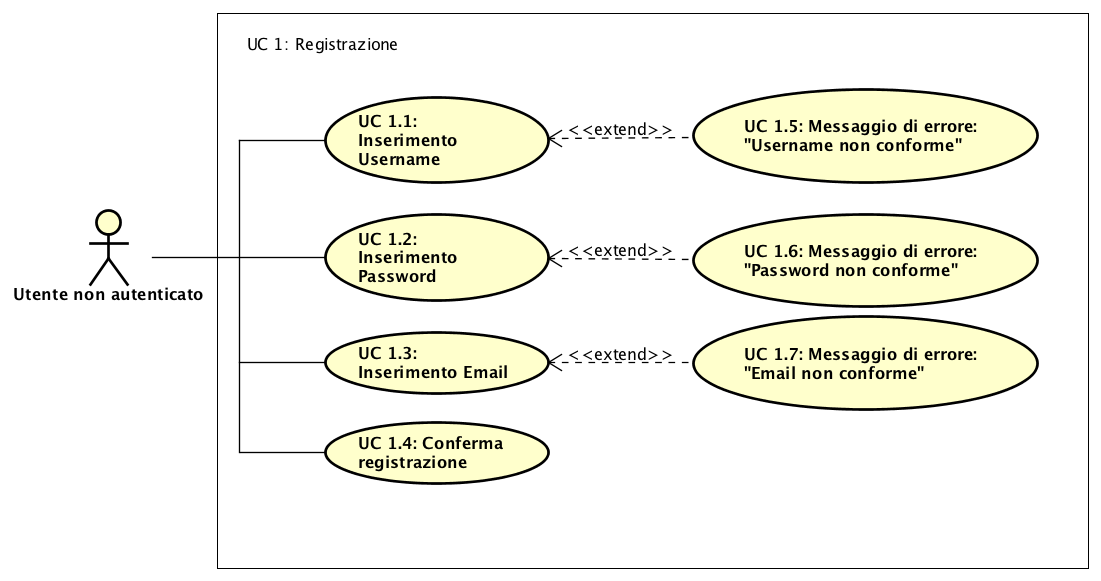
\includegraphics[scale=0.3]{../../Casi D'uso/UC1.png} 
\caption{Caso d'uso UC1} 
 \end{figure} 
\begin{itemize} 
\item \textbf{Attori}: Utente non autenticato.
\item \textbf{Descrizione}: L'attore desidera effettuare l'operazione di registrazione. Vengono richiesti dall'applicazione un username, univoco e conforme alle richieste, una password conforme alle richieste e una mail che rispetti il pattern predefinito;
\item \textbf{Precondizione}: L'applicazione predispone la possibilità di registrazione;
\item \textbf{Postcondizione}: L'applicazione ha creato un nuovo account utente;
\item \textbf{Scenario principale}: \begin{enumerate}\item Inserimento Username (UC1.1);\item Inserimento Password (UC1.2);\item Inserimento Email (UC1.3);\item Conferma registrazione (UC1.4);\item Messaggio di errore: "Username non conforme" (UC1.5);\item Messaggio di errore: "Password non conforme" (UC1.6);\item Messaggio di errore: "Email non conforme" (UC1.7). 
 \end{enumerate}
\item \textbf{Scenari alternativi}: L’attore non autenticato interrompe l’operazione di registrazione non creando un nuovo account.
\end{itemize} 
\subsection{UC1.1 - Inserimento Username} 
\label{ssec:UC1.1} 
\begin{itemize} 
\item \textbf{Attori}: Utente non autenticato.
\item \textbf{Descrizione}: L’attore inserisce l'username: deve essere univoco all'interno dell'applicazione e deve essere alfanumerico;
\item \textbf{Precondizione}: L'applicazione è pronta e l'attore intende autenticarsi;
\item \textbf{Postcondizione}: L'applicazione ha l’informazione relativa all'email inserita dall’utente;
\end{itemize} 
\subsection{UC1.2 - Inserimento Password} 
\label{ssec:UC1.2} 
\begin{itemize} 
\item \textbf{Attori}: Utente non autenticato.
\item \textbf{Descrizione}: L’attore inserisce la password: deve essere di tipo alfanumerico e può contenere caratteri di punteggiatura.;
\item \textbf{Precondizione}: L'attore intende effettuare la registrazione inserendo la password.;
\item \textbf{Postcondizione}: L'attore ha inserito una password conforme alle richieste dell'applicazione.;
\end{itemize} 
\subsection{UC1.3 - Inserimento Email} 
\label{ssec:UC1.3} 
\begin{itemize} 
\item \textbf{Attori}: Utente non autenticato.
\item \textbf{Descrizione}: L’attore inserisce l'email per effettuare la registrazione;
\item \textbf{Precondizione}: L'attore ha selezionato l'opzione di registrazione e non ha ancora inserito un email;
\item \textbf{Postcondizione}: L'applicazione ha l’informazione relativa alla password inserita dall’utente;
\end{itemize} 
\subsection{UC1.4 - Conferma registrazione} 
\label{ssec:UC1.4} 
\begin{itemize} 
\item \textbf{Attori}: Utente non autenticato.
\item \textbf{Descrizione}: Dopo che un attore ha effettuato correttamente una registrazione, ne viene informato;
\item \textbf{Precondizione}: L'attore ha scelto di effettuare l'operazione di registrazione;
\item \textbf{Postcondizione}: L'attore ha ricevuto un messaggio di conferma dell'avvenuta registrazione;
\end{itemize} 
\subsection{UC1.5 - Messaggio di errore: "Username non conforme"} 
\label{ssec:UC1.5} 
\begin{itemize} 
\item \textbf{Attori}: Utente non autenticato.
\item \textbf{Descrizione}: L'attore può inserire un username non conforme e gli viene quindi comunicato l'errore;
\item \textbf{Precondizione}: L'applicazione è pronta e l'utente intende registrarsi;
\item \textbf{Postcondizione}: L'attore ha inserito un username non conforme e ha ricevuto la comunicazione dell'errore;
\end{itemize} 
\subsection{UC1.6 - Messaggio di errore: "Password non conforme"} 
\label{ssec:UC1.6} 
\begin{itemize} 
\item \textbf{Attori}: Utente non autenticato.
\item \textbf{Descrizione}: L'attore può inserire una password non conforme e gli viene quindi comunicato l'errore;
\item \textbf{Precondizione}: L'applicazione è pronta e l'utente intende registrarsi;
\item \textbf{Postcondizione}: L'attore ha inserito una password non conforme e ha ricevuto la comunicazione dell'errore;
\end{itemize} 
\subsection{UC1.7 - Messaggio di errore: "Email non conforme"} 
\label{ssec:UC1.7} 
\begin{itemize} 
\item \textbf{Attori}: Utente non autenticato.
\item \textbf{Descrizione}: L'attore può inserire un'email con una sintassi non valida e gli viene quindi comunicato l'errore;
\item \textbf{Precondizione}: Il sistema è pronto e l'utente intende registrarsi;
\item \textbf{Postcondizione}: L'attore ha inserito un'email non conforme e ha ricevuto la comunicazione dell'errore;
\end{itemize} 
\subsection{UC2 - Autenticazione} 
\label{ssec:UC2} 
\begin{figure}[h!] 
\centering 
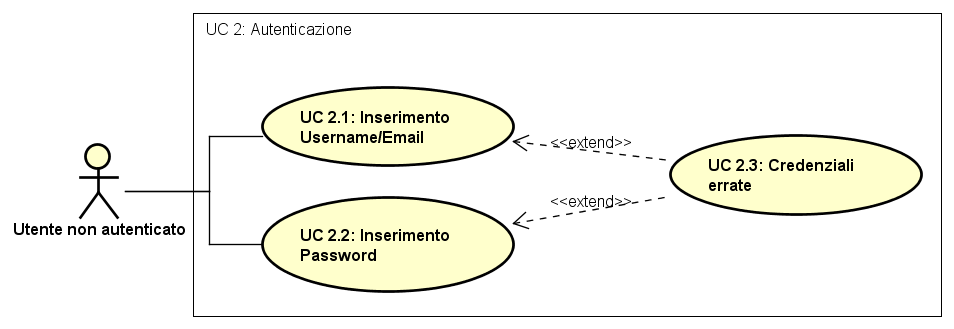
\includegraphics[scale=0.5]{../../Casi D'uso/UC2.png} 
\caption{Caso d'uso UC2} 
 \end{figure} 
\begin{itemize} 
\item \textbf{Attori}: Utente non autenticato.
\item \textbf{Descrizione}: L'attore che già in possesso delle credenziali per accedere all'applicazione, potrà effettuare l'operazione di autenticazione inserendo l'email e la password. Nel caso l’attore abbia perso la password o se la sia dimenticata, l'applicazione fornisce la possibilità di averne una temporanea per poi resettarla;
\item \textbf{Precondizione}: L'attore decide di autenticarsi e l'applicazione richiede l'inserimento dei dati necessari per l'autenticazione;
\item \textbf{Postcondizione}: L'attore ha avuto accesso alle funzionalità del l'applicazione, in caso l'autenticazione sia avvenuta con successo, altrimenti viene visualizzato un messaggio d'errore;
\item \textbf{Scenario principale}: \begin{enumerate}\item Inserimento Username/Email (UC2.1);\item Inserimento Password (UC2.2);\item Password dimenticata (UC2.3);\item Credenziali errate (UC2.4);\item Invio password per email (UC2.5). 
 \end{enumerate}
\item \textbf{Scenari alternativi}: L’attore non effettua l’autenticazione.
\end{itemize} 
\subsection{UC2.1 - Inserimento Username/Email} 
\label{ssec:UC2.1} 
\begin{itemize} 
\item \textbf{Attori}: Utente non autenticato.
\item \textbf{Descrizione}: Durante la fase di autenticazione viene richiesto all'attore il proprio username oppure la propria email;
\item \textbf{Precondizione}: L'applicazione è pronta e l'attore intende autenticarsi;
\item \textbf{Postcondizione}: L'applicazione ha l’informazione relativa all' email/username inserita dall’attore;
\end{itemize} 
\subsection{UC2.2 - Inserimento Password} 
\label{ssec:UC2.2} 
\begin{itemize} 
\item \textbf{Attori}: Utente non autenticato.
\item \textbf{Descrizione}: Durante la fase di autenticazione viene richiesta all'attore la propria password;
\item \textbf{Precondizione}: L'applicazione è pronta e l'attore intende autenticarsi;
\item \textbf{Postcondizione}: L'applicazione ha l’informazione relativa alla password inserita dall’attore
;
\end{itemize} 
\subsection{UC2.3 - Password dimenticata} 
\label{ssec:UC2.3} 
\begin{itemize} 
\item \textbf{Attori}: Utente non autenticato.
\item \textbf{Descrizione}: L'attore ha smarrito oppure ha l'applicazione può fornirgliene una temporanea;
\item \textbf{Precondizione}: L'attore possiede un account all'interno dell'applicazione, ma non è più in possesso della password;
\item \textbf{Postcondizione}: L'attore ha ricevuto una email contenente la nuova password temporanea;
\end{itemize} 
\subsection{UC2.4 - Credenziali errate} 
\label{ssec:UC2.4} 
\begin{itemize} 
\item \textbf{Attori}: Utente non autenticato.
\item \textbf{Descrizione}: L’attore visualizza un messaggio di errore dato dall’inserimento di credenziali errate;
\item \textbf{Precondizione}: L'applicazione ha verificato le credenziali inserite dall’attore;
\item \textbf{Postcondizione}: L'applicazione predispone la visualizzazione di un messaggio di errore;
\end{itemize} 
\subsection{UC2.5 - Invio password per email} 
\label{ssec:UC2.5} 
\begin{itemize} 
\item \textbf{Attori}: Utente non autenticato.
\item \textbf{Descrizione}: Viene inviata una password temporanea all'attore per permettergli di accedere all'applicazione;
\item \textbf{Precondizione}: L'attore richiede una password temporanea;
\item \textbf{Postcondizione}: L'applicazione ha inviato all'attore una mail contenente la password temporanea;
\end{itemize} 
\subsection{UC3 - Gestione Profilo} 
\label{ssec:UC3} 
\begin{itemize} 
\item \textbf{Attori}: Utente Autenticato.
\item \textbf{Descrizione}: L' attore può gestire il suo username, la sua password o il suo indirizzo email;
\item \textbf{Precondizione}: L' attore ha già effettuato l'accesso e l'applicazione rende disponibile la voce Gestione Profilo nel menù;
\item \textbf{Postcondizione}: L' applicazione visualizza i dati dell'attore con gli opportuni pulsanti di modifica;
\item \textbf{Scenario principale}: \begin{enumerate}\item Modifica Username (UC3.1);\item Modifica Password (UC3.2);\item Modifica Email (UC3.3);\item Eliminazione Profilo (UC3.4);\item Messaggio di errore: "Username non conforme" (UC3.5);\item Messaggio di errore: "Password non conforme" (UC3.6);\item Messaggio di errore: "Email non conforme" (UC3.7). 
 \end{enumerate}
\end{itemize} 
\subsection{UC3.1 - Modifica Username} 
\label{ssec:UC3.1} 
\begin{itemize} 
\item \textbf{Attori}: Utente Autenticato.
\item \textbf{Descrizione}: L' attore può modificare il suo username;
\item \textbf{Precondizione}: L'  attore vuole modificare l'username;
\item \textbf{Postcondizione}: L' applicazione modifica l' username dell'attore;
\item \textbf{Scenari alternativi}: L' attore annulla la modifica dell'username.
\end{itemize} 
\subsection{UC3.2 - Modifica Password} 
\label{ssec:UC3.2} 
\begin{itemize} 
\item \textbf{Attori}: Utente Autenticato.
\item \textbf{Descrizione}: L' attore ha la possibilità di modificare la sua password;
\item \textbf{Precondizione}: L'  attore vuole modificare la password;
\item \textbf{Postcondizione}: L' applicazione modifica la password o restituisce il messaggio d'errore;
\item \textbf{Scenari alternativi}: L' attore annulla la modifica della password.
\end{itemize} 
\subsection{UC3.3 - Modifica Email} 
\label{ssec:UC3.3} 
\begin{itemize} 
\item \textbf{Attori}: Utente Autenticato.
\item \textbf{Descrizione}: L' attore ha la possibilità di modificare la propria email;
\item \textbf{Precondizione}: L' attore vuole modificare l'email;
\item \textbf{Postcondizione}: L' applicazione aggiorna l'email;
\item \textbf{Scenari alternativi}: L' attore annulla la modifica dell'email.
\end{itemize} 
\subsection{UC3.4 - Eliminazione Profilo} 
\label{ssec:UC3.4} 
\begin{itemize} 
\item \textbf{Attori}: Utente Autenticato.
\item \textbf{Descrizione}: L'attore può eliminare il profilo, cancellando ogni tipo di personalizzazione da lui creata;
\item \textbf{Precondizione}: L'applicazione permette l'eliminazione del profilo;
\item \textbf{Postcondizione}: L'applicazione ha cancellato a cascata ogni informazione legata a tale profilo ed essa non è più recuperabile;
\item \textbf{Scenari alternativi}: L'attore annulla la cancellazione del profilo.
\end{itemize} 
\subsection{UC3.5 - Messaggio di errore: "Username non conforme"} 
\label{ssec:UC3.5} 
\begin{itemize} 
\item \textbf{Attori}: Utente Autenticato.
\item \textbf{Descrizione}: L'attore può inserire un username non conforme e gli viene quindi comunicato l'errore;
\item \textbf{Precondizione}: L'applicazione è pronta e l'utente modificare l'username;
\item \textbf{Postcondizione}: L'attore ha inserito un username non conforme e ha ricevuto la comunicazione dell'errore;
\end{itemize} 
\subsection{UC3.6 - Messaggio di errore: "Password non conforme"} 
\label{ssec:UC3.6} 
\begin{itemize} 
\item \textbf{Attori}: Utente Autenticato.
\item \textbf{Descrizione}: L'attore può inserire una password non conforme e gli viene quindi comunicato l'errore;
\item \textbf{Precondizione}: L'applicazione è pronta e l'utente modificare la password;
\item \textbf{Postcondizione}: L'attore ha inserito una password non conforme e ha ricevuto la comunicazione dell'errore;
\end{itemize} 
\subsection{UC3.7 - Messaggio di errore: "Email non conforme"} 
\label{ssec:UC3.7} 
\begin{itemize} 
\item \textbf{Attori}: Utente Autenticato.
\item \textbf{Descrizione}: L'attore può inserire l'email con una sintassi non valida e gli viene quindi comunicato l'errore;
\item \textbf{Precondizione}: Il sistema è pronto e l'utente intende modificare l'email;
\item \textbf{Postcondizione}: L'attore ha inserito un'email non conforme e ha ricevuto la comunicazione dell'errore;
\end{itemize} 
\subsection{UC4 - Logout} 
\label{ssec:UC4} 
\begin{itemize} 
\item \textbf{Attori}: Utente Autenticato.
\item \textbf{Descrizione}: L' attore può effettuare il logout dal suo profilo;
\item \textbf{Precondizione}: L’applicazione mette a disposizione dell’attore la possibilità di logout;
\item \textbf{Postcondizione}: L' applicazione effettua il logout dell'attore;
\end{itemize} 
\subsection{UC5 - Gestione Progetti} 
\label{ssec:UC5} 
\begin{itemize} 
\item \textbf{Attori}: Utente Autenticato.
\item \textbf{Descrizione}: L’ attore ha la possibilità di aggiungere un nuovo progetto e di aprire o modificare un progetto già esistente;
\item \textbf{Precondizione}: L'applicazione è pronta e l'attore intende gestire un progetto;
\item \textbf{Postcondizione}: L’ applicazione visualizza la lista delle funzionalità disponibili;
\item \textbf{Scenario principale}: \begin{enumerate}\item Aggiunta Progetto (UC5.1);\item Apertura progetto (UC5.2);\item Eliminazione Progetto (UC5.3). 
 \end{enumerate}
\end{itemize} 
\subsection{UC5.1 - Aggiunta Progetto} 
\label{ssec:UC5.1} 
\begin{itemize} 
\item \textbf{Attori}: Utente Autenticato.
\item \textbf{Descrizione}: L’attore ha la possibilità di creare o importare un progetto;
\item \textbf{Precondizione}: L’attore vuole aggiungere un nuovo progetto alla lista;
\item \textbf{Postcondizione}: L’applicazione apre la lista dei modi per aggiungere un progetto;
\item \textbf{Scenario principale}: \begin{enumerate}\item Creazione Progetto vuoto (UC5.1.1);\item Importazione Progetto (UC5.1.2). 
 \end{enumerate}
\item \textbf{Scenari alternativi}: L'attore decide di non aggiungere un nuovo progetto.
\end{itemize} 
\subsection{UC5.1.1 - Creazione Progetto vuoto} 
\label{ssec:UC5.1.1} 
\begin{itemize} 
\item \textbf{Attori}: Utente Autenticato.
\item \textbf{Descrizione}: L'attore può creare un nuovo progetto;
\item \textbf{Precondizione}: L'attore vuole creare un progetto vuoto;
\item \textbf{Postcondizione}: L'applicazione crea un nuovo progetto vuoto;
\item \textbf{Scenari alternativi}: L'attore annulla la creazione del nuovo progetto.
\end{itemize} 
\subsection{UC5.1.2 - Importazione Progetto} 
\label{ssec:UC5.1.2} 
\begin{itemize} 
\item \textbf{Attori}: Utente Autenticato.
\item \textbf{Descrizione}: L'attore può importare un progetto;
\item \textbf{Precondizione}: L' attore vuole importare un progetto;
\item \textbf{Postcondizione}: L'applicazione importa il progetto richiesto;
\item \textbf{Scenari alternativi}: L'attore decide di non importare nessun progetto.
\end{itemize} 
\subsection{UC5.2 - Apertura progetto} 
\label{ssec:UC5.2} 
\begin{itemize} 
\item \textbf{Attori}: Utente Autenticato.
\item \textbf{Descrizione}: L’ attore ha la possibilità di aprire un progetto precedentemente salvato.;
\item \textbf{Precondizione}: L’ applicazione rende disponibile la lista dei progetti dell'attore;
\item \textbf{Postcondizione}: L’applicazione apre il progetto selezionato;
\end{itemize} 
\subsection{UC5.3 - Eliminazione Progetto} 
\label{ssec:UC5.3} 
\begin{itemize} 
\item \textbf{Attori}: Utente Autenticato.
\item \textbf{Descrizione}: L' attore ha la possibilità di eliminare un progetto precedentemente salvato;
\item \textbf{Precondizione}: L’applicazione rende disponibile la lista dei progetti salvati dall'attore;
\item \textbf{Postcondizione}: L’applicazione elimina il progetto selezionato;
\end{itemize} 
\subsection{UC6 - Tool Designer} 
\label{ssec:UC6} 
\begin{itemize} 
\item \textbf{Attori}: Utente Autenticato.
\item \textbf{Descrizione}: L'applicazione visualizza l'editor dei diagrammi;
\item \textbf{Precondizione}: L' attore ha effettuato l'accesso;
\item \textbf{Postcondizione}: L'applicazione visualizza la finestra;
\item \textbf{Scenario principale}: \begin{enumerate}\item Menù (UC6.1);\item Barra degli strumenti (UC6.2);\item Disegnatore diagrammi (UC6.3);\item Pannello laterale (UC6.4). 
 \end{enumerate}
\end{itemize} 
\subsection{UC6.1 - Menù} 
\label{ssec:UC6.1} 
\begin{itemize} 
\item \textbf{Attori}: Utente Autenticato.
\item \textbf{Descrizione}: L’ attore può accedere alle voci file, edit, tool,
layers e window appartenenti al menù del tool designer;
\item \textbf{Precondizione}: L’applicazione offre all’utente una barra dei menù;
\item \textbf{Postcondizione}: L’applicazione, a seconda dell’operazione richiesta dall’utente,
svolge le sue funzioni;
\item \textbf{Scenario principale}: \begin{enumerate}\item File (UC6.1.1);\item Edit (UC6.1.2);\item Template (UC6.1.3);\item Layers (UC6.1.4). 
 \end{enumerate}
\end{itemize} 
\subsection{UC6.1.1 - File} 
\label{ssec:UC6.1.1} 
\begin{itemize} 
\item \textbf{Attori}: Utente Autenticato.
\item \textbf{Descrizione}: L’attore può accedere alle voci salva, chiudi, esporta, genera codice e salva template appartenenti alla voce file del menù;
\item \textbf{Precondizione}: L’applicazione offre all’utente la voce file nella barra dei menù;
\item \textbf{Postcondizione}: L’applicazione, a seconda dell’operazione richiesta dall’utente,
svolge le sue funzioni;
\item \textbf{Scenario principale}: \begin{enumerate}\item Salvataggio (UC6.1.1.1);\item Chiusura (UC6.1.1.2);\item Esportazione (UC6.1.1.3);\item Genera codice (UC6.1.1.4);\item Salvataggio template (UC6.1.1.5). 
 \end{enumerate}
\end{itemize} 
\subsection{UC6.1.1.1 - Salvataggio} 
\label{ssec:UC6.1.1.1} 
\begin{itemize} 
\item \textbf{Attori}: Utente Autenticato.
\item \textbf{Descrizione}: L’attore può salvare il suo progetto nello stato corrente;
\item \textbf{Precondizione}: L’attore ha aperto un progetto;
\item \textbf{Postcondizione}: L’applicazione salva il progetto nello stato corrente;
\end{itemize} 
\subsection{UC6.1.1.2 - Chiusura} 
\label{ssec:UC6.1.1.2} 
\begin{itemize} 
\item \textbf{Attori}: Utente Autenticato.
\item \textbf{Descrizione}: L’attore può chiudere il progetto corrente;
\item \textbf{Precondizione}: L'attore ha aperto un progetto;
\item \textbf{Postcondizione}: L’applicazione chiude il progetto corrente;
\end{itemize} 
\subsection{UC6.1.1.3 - Esportazione} 
\label{ssec:UC6.1.1.3} 
\begin{itemize} 
\item \textbf{Attori}: Utente Autenticato.
\item \textbf{Descrizione}: L’attore può esportare il progetto corrente per possederne una copia digitale;
\item \textbf{Precondizione}: L’attore ha un progetto aperto;
\item \textbf{Postcondizione}: L’applicazione esporta il progetto in un formato compresso;
\end{itemize} 
\subsection{UC6.1.1.4 - Genera codice} 
\label{ssec:UC6.1.1.4} 
\begin{itemize} 
\item \textbf{Attori}: Utente Autenticato.
\item \textbf{Descrizione}: L’attore può generare il codice relativo all’UML prodotto;
\item \textbf{Precondizione}: L’attore vuole generare il codice dai suoi diagrammi UML;
\item \textbf{Postcondizione}: L’applicazione genera il codice relativo al disegno UML;
\end{itemize} 
\subsection{UC6.1.1.5 - Salvataggio template} 
\label{ssec:UC6.1.1.5} 
\begin{itemize} 
\item \textbf{Attori}: Utente Autenticato.
\item \textbf{Descrizione}: L’attore ha la possibilità di salvare determinate classi o gerarchie, aggiungendole così alla lista di template già salvati;
\item \textbf{Precondizione}: L’applicazione offre all’attore la voce salva template, sottovoce di file nel menù, solamente se sono state create una o più classi, ed ognuna di esse ha un commento che le identifica;
\item \textbf{Postcondizione}: Viene aggiunto alla lista dei template il template desiderato;
\end{itemize} 
\subsection{UC6.1.2 - Edit} 
\label{ssec:UC6.1.2} 
\begin{itemize} 
\item \textbf{Attori}: Utente Autenticato.
\item \textbf{Descrizione}: L’attore può accedere alle voci annulla, ripristina, taglia, copia, incolla, zoom in e zoom out appartenenti alla voce edit del menù;
\item \textbf{Precondizione}: L'attore ha aperto un progetto;
\item \textbf{Postcondizione}: L’applicazione visualizza la lista delle funzionalità disponibili;
\item \textbf{Scenario principale}: \begin{enumerate}\item Annulla (UC6.1.2.1);\item Ripristina (UC6.1.2.2);\item Taglia (UC6.1.2.3);\item Copia (UC6.1.2.4);\item Incolla (UC6.1.2.5);\item Zoom in (UC6.1.2.6);\item Zoom out (UC6.1.2.7). 
 \end{enumerate}
\end{itemize} 
\subsection{UC6.1.2.1 - Annulla} 
\label{ssec:UC6.1.2.1} 
\begin{itemize} 
\item \textbf{Attori}: Utente Autenticato.
\item \textbf{Descrizione}: L’attore può tornare allo stato precedente l’ultima modifica;
\item \textbf{Precondizione}: L'attore ha un progetto aperto e ne ha effettuato una modifica;
\item \textbf{Postcondizione}: L’applicazione torna allo stato precedente l’ultima modifica;
\end{itemize} 
\subsection{UC6.1.2.2 - Ripristina} 
\label{ssec:UC6.1.2.2} 
\begin{itemize} 
\item \textbf{Attori}: Utente Autenticato.
\item \textbf{Descrizione}: L’attore può ripristinare le modifiche effettuate successivamente allo stato attuale;
\item \textbf{Precondizione}: L’attore ha un progetto aperto ed ha annullato una modifica (UC 6.1.2.1);
\item \textbf{Postcondizione}: L’applicazione torna allo stato precedente l’ultima modifica;
